\documentclass{article}
\usepackage{amsmath}
\usepackage{caption}
\captionsetup[figure]{name=Gambar}
\usepackage{graphicx}
\begin{document}

Nama: Rifqi Fadil Fahrial \newline
NIM: 1222646 \newline



\begin{figure}
  \begin{center}
    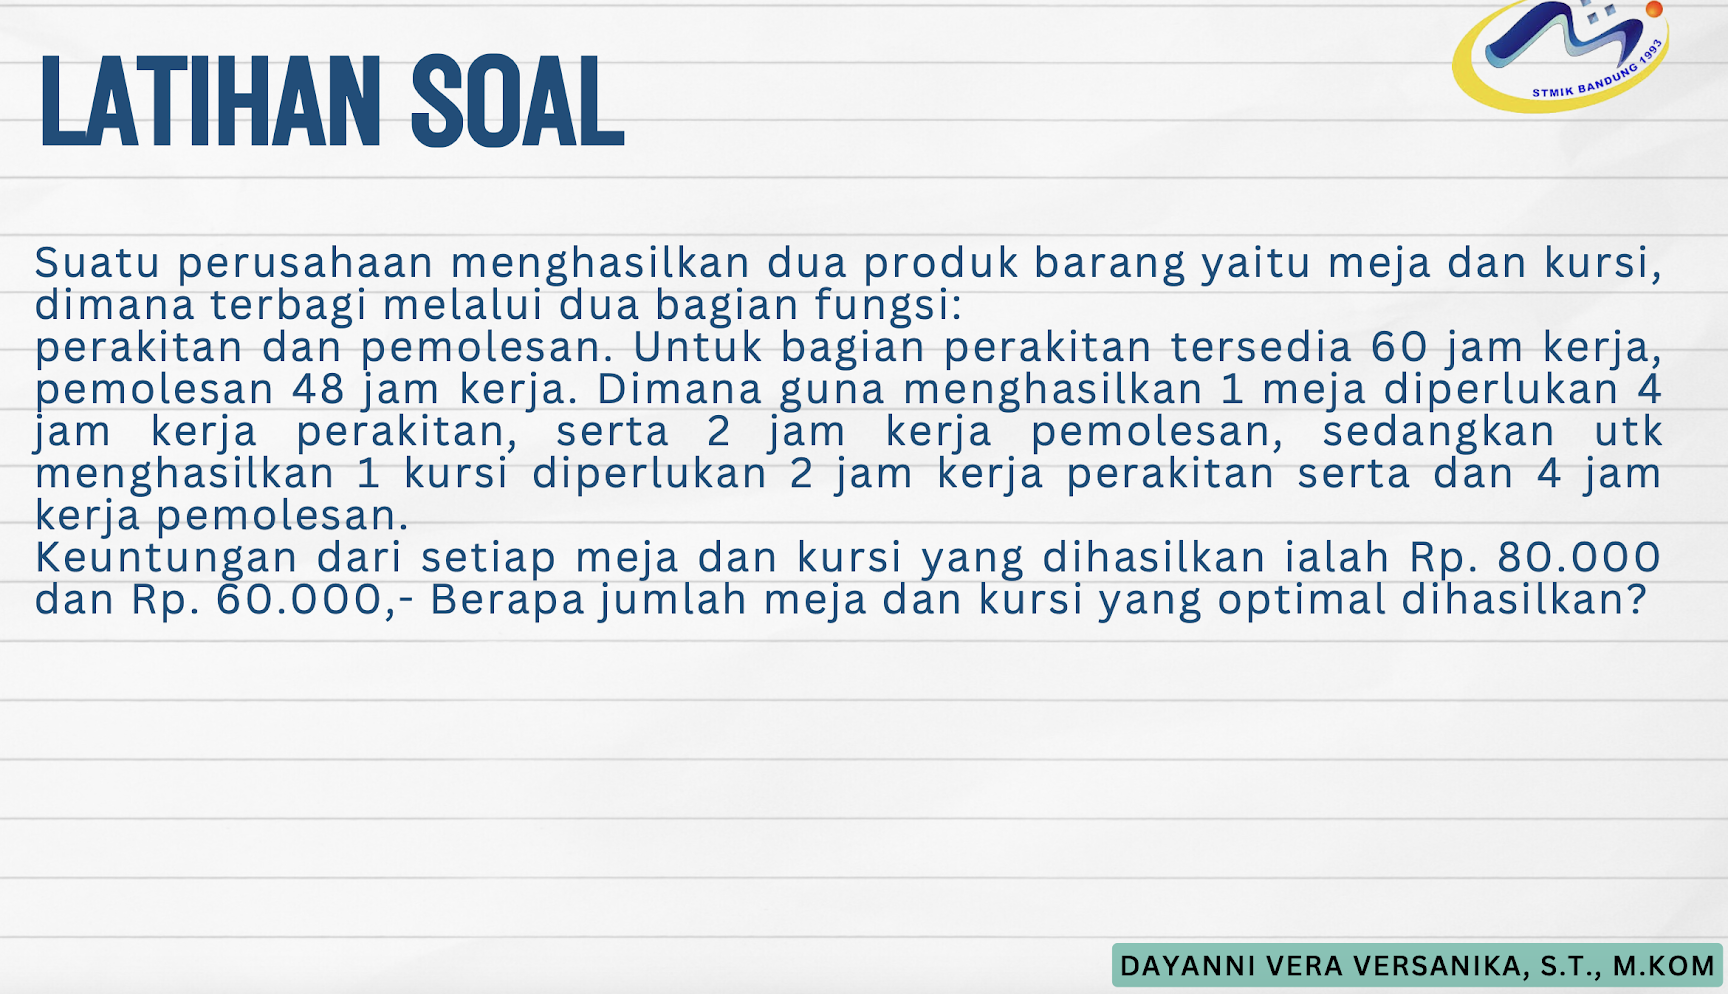
\includegraphics[width=0.95\textwidth]{images/gambar.png}
  \end{center}
  \caption{Soal}
\end{figure}



\subsection*{Langkah 1: Definisikan Variabel}
\begin{itemize}
    \item \( x \) = jumlah meja yang diproduksi
    \item \( y \) = jumlah kursi yang diproduksi
\end{itemize}

\subsection*{Langkah 2: Definisikan Fungsi Tujuan}
Keuntungan dari setiap meja adalah Rp 80.000 dan dari setiap kursi adalah Rp 60.000. Fungsi tujuan yang ingin dimaksimalkan adalah:
\[
\text{Keuntungan} = 80.000x + 60.000y
\]

\subsection*{Langkah 3: Definisikan Batasan}
\begin{enumerate}
    \item \textbf{Batasan Waktu Perakitan:}
    \[
    4x + 2y \leq 60
    \]
    
    \item \textbf{Batasan Waktu Pemolesan:}
    \[
    2x + 4y \leq 48
    \]
    
    \item \textbf{Batasan Non-Negatif:}
    \[
    x \geq 0, \quad y \geq 0
    \]
\end{enumerate}

\subsection*{Langkah 4: Selesaikan Sistem Persamaan}
mencari titik potong kedua garis
\[
4x + 2y = 60
\]
\[
2x + 4y = 48
\]

Sederhanakan persamaan pertama 
\[
2x + y = 30
\]
\[
y = 30 - 2x
\]

Substitusi \( y \) ke dalam persamaan kedua:
\[
2x + 4(30 - 2x) = 48
\]
\[
2x + 120 - 8x = 48
\]
\[
-6x = -72
\]
\[
x = 12
\]

Substitusi \( x = 12 \) ke dalam persamaan \( y = 30 - 2x \):
\[
y = 30 - 2(12) = 6
\]

\begin{figure}[ht]
  \begin{center}
    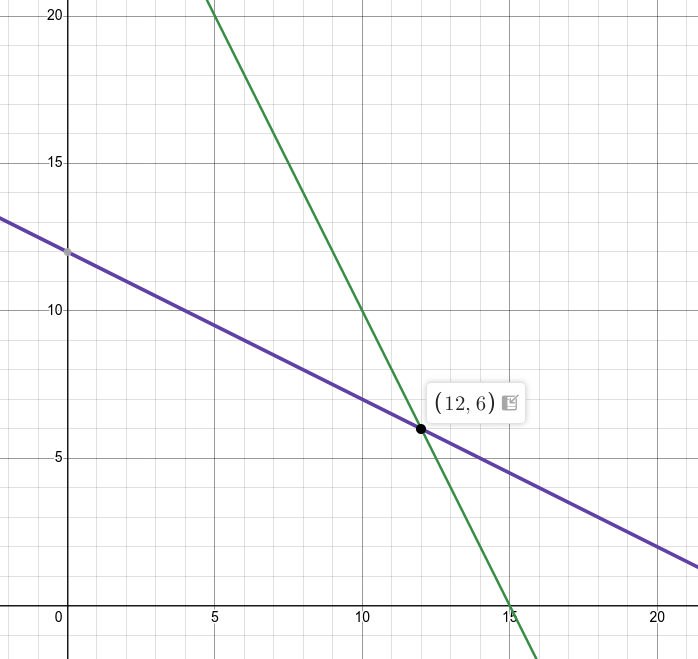
\includegraphics[width=0.5\textwidth]{images/graph.png}
  \end{center}
  \caption{Grafik}\label{Grafik}
\end{figure}


\subsection*{Langkah 5: Hitung Keuntungan}
\[
\text{Keuntungan} = 80.000(12) + 60.000(6)
\]
\[
\text{Keuntungan} = 960.000 + 360.000 = 1.320.000
\]

\subsection*{Kesimpulan}
Jumlah optimal yang harus diproduksi adalah \textbf{12 meja} dan \textbf{6 kursi} dengan keuntungan maksimal sebesar \textbf{Rp 1.320.000}.

\end{document}
